%%%%%%%%%%%%%%%%%%%%%%%%%%%%%%%%%%%%%%%%%%%%%%%%%%%%%%%%%%%%%%%%%%%%%%%%%%%%%%%%
% Лабораторная работа 7 : Принцип Сен Венана

% Выполнили             : Баталов Семен, Хайретдинова Диана, 2021.
%%%%%%%%%%%%%%%%%%%%%%%%%%%%%%%%%%%%%%%%%%%%%%%%%%%%%%%%%%%%%%%%%%%%%%%%%%%%%%%%

\documentclass[12pt, a4paper]{article}
\usepackage[left=1.5cm, right=2cm, top=2.5cm, bottom=2.5cm, nohead]{geometry}
\usepackage{graphicx}
\usepackage[utf8]{inputenc}
\usepackage[english, russian]{babel}
\usepackage{indentfirst}
\usepackage{amsmath}
\usepackage{longtable}
\usepackage{multirow}
\usepackage{array}
\usepackage{rotating}
\usepackage{subcaption}
\graphicspath{{./Pictures/}}

\begin{document}
    
    \newcolumntype{M}[1]{>{\centering\arraybackslash}m{#1}}
    \renewcommand{\arraystretch}{1.3}
    
    \begin{center}
        \large{Санкт-Петербургский Государственный Университет} \\
        \large{Saint-Petersburg State University}\\
        \hfill \break
        \hfill \break
        \hfill \break
        \hfill \break
        \hfill \break
        \hfill \break
        \large{ЛАБОРАТОРИЯ ПРОЧНОСТИ МАТЕРИАЛОВ} \\
        \hfill \break
        \hfill \break
        \hfill \break
        \large{\textbf{ОТЧЕТ}} \\
        \large{\textbf{По лабораторной работе 7}} \\
        \large{<<Принцип Сен-Венана>>} \\
        \hfill \break
        \hfill \break
        \hfill \break
        \large{По дисциплине} \\
        \large{<<Лабораторный практикум, лабораторная работа>>} \\
    \end{center}
    
    \hfill \break
    \hfill \break
    \hfill \break
    \hfill \break
    \hfill \break
    \hfill \break
    
    \begin{flushright} 
        \large{Выполнили:} \\
        \hfill \break
        \large{Баталов С. А.} \\
        \large{Хайретдинова Д. Д.} \\
    \end{flushright}
    
    \hfill \break
    \hfill \break
    \hfill \break
    \hfill \break
    \hfill \break
    
    \begin{center} 
        \large{Санкт-Петербург} \\
        \large{2021} \\
    \end{center}
    
    \thispagestyle{empty}
    \newpage
    \sloppy
    
    \section{Цель работы}
	Принцип Сен-Венана - один из основополагающих принципов механики. Он не имеет строгого доказательства в общем виде, но подтверждается многочисленными экспериментами, а также решениями частных задач.

 Принцип Сен-Венана позволяет принимать во внимание лишь равнодействующие внешних сил, не рассматривая особенности их приложения.
	
	Цель работы заключается в иллюстрации принципа Сен-Венана.
    
    \newpage
    \section{Теоретическое исследование и Экспериментальная установка}
    Согласно принципу Сен-Венана, особенности приложения внешних сил, как правило, проявляются в непосредственной близости от места их приложения. Применительно к растянутому стержню эти особенности не превышают характерных размеров поперечного сечения.
    
	Краевые особенности создаются путем различного раскроя концов резиновых полос. Различные устройства <<законцовок>>  позволяют реализовать разные схемы передачи нагрузки на стержень и приложить три разные, но статически эквивалентные системы внешних сил. В первом случае (\ref{rezinochki}, слева) н\ref{rezinochki}, в центре) - сосредоточена в центре, в третьем (\ref{rezinochki}, справа) - сосредоточена по краям.
    
    \begin{figure}[h]
\centering
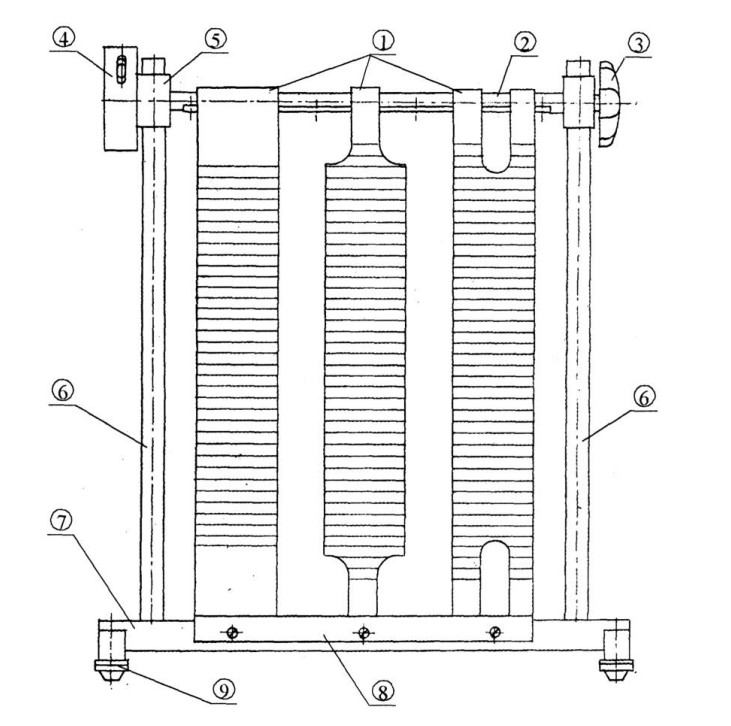
\includegraphics[width = 15cm]{modelka.jpg}
\caption{Демонстрационная модель М1}
\label{rezinochki}
\end{figure}
	Демонстрационная модель состоит из 3 резиновых полос с отличающимися раскроями швов $1$, поворотного устройства с эксцентричным влом $2$, маховиками $3$ и $4$, хомутами $5$. Также в нее входят силовой рамы $7$, стойки $6$, траверса $2$ , прижимные пластины $8$ и элементы горизонтирования $9$.
	В данной работе нагрузка осуществляется вращением маховиков 1 и 2 полных оборота.
    \newpage
    \section{Эксперимент}
    Замерили геометрические размеры трех лент : длину лент $l$ , ширину лент $d$ и среднее расстояние между линиями сетки $h$; также посчитали размеры области приложения нагрузки $S$ -- на первой ленте $S = d^2$, на второй ленте --  $S = d_{2}^2$, на третьей ленте $S = 2\cdot (d_{3})^2$, где $d_{2}$ и $d_{3}$ ширины тонкой полосы 2 и 3 лент.
    
 \begin{table}[h]
 	\centering
 	\begin{tabular}{|M{2cm}|M{2cm}|M{2cm}|M{2cm}|M{2.5cm}|}
 		\hline
 		\multirow{2}{*}{Величина} & \multicolumn{3}{c|}{Значение} & \multirow{2}{*}{Размерность} \\
 		\cline{2-4}
 		& 1 & 2 & 3 & \\
 		\hline
 		$l$ & 460 $\pm$ 1 & 460 $\pm$ 1  & 460 $\pm$ 1 & \multirow{3}{*}{мм} \\
 		$d$ & 56 $\pm$ 1 & 55 $\pm$ 1  & 55 $\pm$ 1 & \\
 		$h$ & 9 $\pm$ 1 & 9 $\pm$ 1  & 9 $\pm$ 1 & \\
 		\hline
 		$S$ & 2927 $\pm$ 116 & 625 $\pm$ 50  & 650 $\pm$ 72 & мм$^2$ \\
 		\hline
 	\end{tabular}
 	\caption{Начальные данные}
 \end{table}
 	Растягивая ленты путем вращения эксцентричного вала за маховики, измерили среднее расстояние между линиями сетки $h$ в центре лент и размеров области нагружения $d$ и $S$ -- размеры области приложения нагрузки при 1 и 2 полных оборотах:
 	 \begin{table}[h]
 	\centering
 	\begin{tabular}{|M{1cm}|M{2cm}|M{2cm}|M{2cm}|M{2cm}|M{2.5cm}|}
 		\hline
 		\multirow{2}{*}{№} &  \multirow{2}{*}{Величина} & \multicolumn{3}{c|}{Значение} & \multirow{2}{*}{Размерность} \\
 		\cline{3-5}
 		& & 1 & 2 & 3 & \\
 		\hline
 		1 & $d$ & 52 $\pm$ 1 & 53 $\pm$ 1  & 53 $\pm$ 1 & \multirow{2}{*}{мм} \\
 		& $h$ & 10 $\pm$ 1 & 10 $\pm$ 1  & 10 $\pm$ 1 & \\
 		\cline{2-6}
 		& $S$ & 2810 $\pm$ 106 & 485 $\pm$ 44  & 512 $\pm$ 72 & мм$^2$ \\

 		\hline
 		2 & $d$ & 50 $\pm$ 1 & 52 $\pm$ 1  & 52 $\pm$ 1 & \multirow{2}{*}{мм} \\
 		& $h$ & 11 $\pm$ 1 & 11 $\pm$ 1  & 11 $\pm$ 1 & \\
 		\cline{2-6}
 		& $S$ & 2500 $\pm$ 100 & 400 $\pm$ 40  & 392 $\pm$ 56 & мм$^2$\\
 		\hline
 		
 	\end{tabular}
 	\caption{Экспериментальные данные.}
 \end{table}
	
	Зарисовали картину деформирования делительных сетк вблизи вырезов после каждого оборота маховика:
	
 \begin{figure}[h!]
\centering
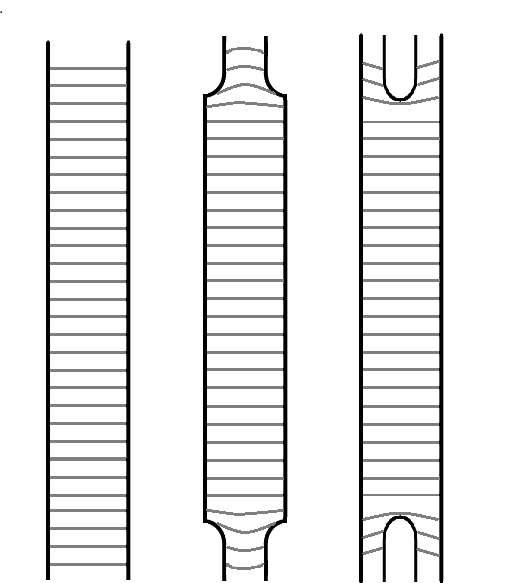
\includegraphics[width = 9.5cm]{omg_1.png}
\caption{Вид полос при 1 обороте}
\label{pic}
\end{figure} 
\hfill

    \begin{figure}[h!]
\centering
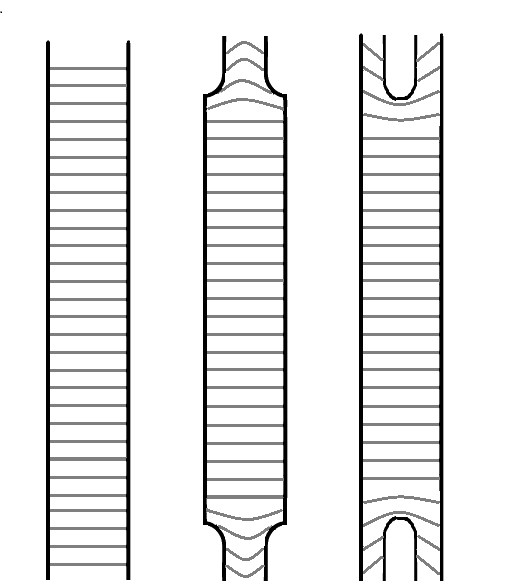
\includegraphics[width = 9.5cm]{omg_2.png}
\caption{Вид полос при 2 оборотах}
\label{one_more_pic}
\end{figure}


\newpage 	 

\section{Вывод}

	В данной работе познакомились с работой принципа Сен-Венана и убедились в его экспериментальной  справедливости. При растяжении эквивалентными силами лент с разными законцовками горизонтальные полосы влизи этих законцовок деформируются неодинаково.
	
	Деформирование происходит только по краям полос и эти краевые особенности быстро затухают на длине,соответствующей характерному размеру поперечному сечения ленты.
\end{document}
